\chapter{Realisierung}

\section{Systemübersicht}

\begin{figure}[H]
	\centering
	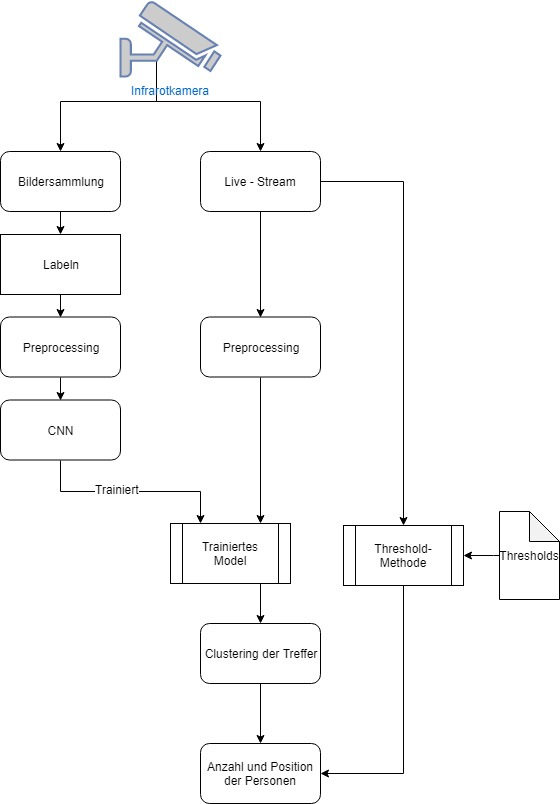
\includegraphics[width=.8\linewidth]{SystemOverview}
	\caption{Grobübersicht des Systems mit CNN- und Thresholdalgorithmus}
	\label{SystemOverview}
\end{figure}

\section{UDP-Schnittstelle}

Um die Bilder automatisiert erhalten zu können wurde eine Schnittstelle zu den Infrarotkameras implementiert. Es wurde das UDP-Protokoll verwendet, da die Kameras nur über dieses Protokoll angesprochen werden konnten.\\
 Die einzige ander Möglichkeit and Bilder zu gelangen wäre über die GUI Applikation des Herstellers Videos aufzunehmen. Dies sind bereits auf RGB convertiert, beihalten also nicht alle Information des ursprünglichen Bildes und die Applikation kann nicht automatisiert angesprochen werden. Folglich ist dies keine praktikable Variante um effizient Daten zu sammeln.\\
\\
Die Kameras können ausserdem nur mittels UDP-Broadcasts identifiziert und and einen Socket gebunden werden. Aus diesem Grund konnten die Kameras nicht im allgemeinen Schulnetzwerk installiert werden, sondern mussten in einem separaten Netzwerk betrieben werden. In diesem Netzwerk konnten sie über einen Computer angesteuert werden, der widerum mit dem HSLU-Netzwerk verbunden ist. Um die Entwicklung der Schnittstelle möglichst einfach zu gestalten wurde versucht einen Remoteinterpreter aufzusetzen. Dies ist eine funktion von Pycharm \parencite{pycharm} erlaubt es, auf einem Lokalen System zu entwickeln aber die Software direkt auf einem Remote System auszuführen und zu Debuggen.\\
Leider wird dies für Windows Remote Systeme nicht unterstützt. Deshalb wurde der Code jeweils manuell via sftp auf den Computer im Sitzungszimmer kopiert. Danach wurde mittel Windows Remotedesktopverbindung die Software ausgeführt und getestet. \\
\\
In einer ersten Variante wurde in dieser Schnittstelle mit Einzelbilder gearbeitet. Dies bietet den Vorteil, dass man die Bildrate einfah definieren und steuern kann. Leider war die Qualitiät dieser Bilder sehr schlecht. Durch eine Rücksprach mit dem Hersteller stellte sich heraus, das die Verwendung der Streaming Funktion der Kameras qualitativ besser Bilder liefert. Deshalb wurde die Schnittstelle auf die Verwendung von Streams abgeändert. Dabei war die Generator Funktionalität von Python sehr hilfreich. Die Eigenschaft von Generators, dass diese erst ausgeführt werden, wenn ein Objekt angefragt wird, konnte genutzt werden, um jederzeit das aktuellste Bild zu erhalten.

\section{Datensammlung}

Um die Trainingsdaten effizient zu sammeln wurde ein  Skript erstellt, welches von beiden Kameras gleichzeitig Bilder anfordert und Abspeichert. Dieses musste über mehrere Monate unterbruchlos laufen und wurde deshalb so Implementiert, dass es sich bei einem Fehler automatisch neu startet. Zusätzlich wurden parallel dazu auch Bilder der Referenzkamera aufgezeichnet, um das Labeling der Infrarotbilder zu vereinfachen und als Ground Truth zu verifizieren.\\
Alle aufgezeichneten Bilder wurden lokal auf einer Festplatte des Computers im Sitzungszimmer gespeichert. Um alle Bilder eindeutig zu identifizieren, wurden sie mit Art des Bildes, Infrarot oder Ground Truth, Zeitstempel und bei den Infrarotbildern mit Kamera 1 oder 2 versehen. Um das ganze übersichtlicher zu gestalten wurde das ganze in einem Ordnersystem abgelegt, das wie folgt aufgebaut ist.

\begin{itemize}
	\item ../ [Jahr] / [Monat] / [Tag] / [Bildtyp]\_[Uhrzeit]\_[Kamera].[Dateityp]
	\item Bsp.: ../2019/05/23/IR\_Image\_10\_33\_45\_2.npy
\end{itemize}


\section{Algorithmen}

Damit die beiden Algorithmen möglichst effizient und mit wenig Redundanz implementierte werden konnten, wurde die Software modular aufgebaut. 



